\documentclass[10pt]{report}
\usepackage[centertags]{amsmath}
\usepackage{amsfonts}
\usepackage{amssymb}
\usepackage{amsthm}
\usepackage{newlfont}
\usepackage{graphicx}
%\usepackage[super,sort&compress]{natbib}
%\usepackage[sort&compress]{natbib}
%\usepackage[numbers]{natbib}
\usepackage[authoryear,square]{natbib}

\hfuzz2pt
\newlength{\defbaselineskip}
\setlength{\defbaselineskip}{\baselineskip}
\newcommand{\setlinespacing}[1]%
           {\setlength{\baselineskip}{#1 \defbaselineskip}}
\newcommand{\doublespacing}{\setlength{\baselineskip}%
                           {2.0 \defbaselineskip}}
\newcommand{\singlespacing}{\setlength{\baselineskip}{\defbaselineskip}}
\newcommand{\A}{{\cal A}}
\newcommand{\h}{{\cal H}}
\newcommand{\s}{{\cal S}}
\newcommand{\W}{{\cal W}}
\newcommand{\BH}{\mathbf B(\cal H)}
\newcommand{\KH}{\cal  K(\cal H)}
\newcommand{\Real}{\mathbb R}
\newcommand{\Complex}{\mathbb C}
\newcommand{\Field}{\mathbb F}
\newcommand{\RPlus}{[0,\infty)}
\newcommand{\norm}[1]{\left\Vert#1\right\Vert}
\newcommand{\essnorm}[1]{\norm{#1}_{\text{\rm\normalshape ess}}}
\newcommand{\abs}[1]{\left\vert#1\right\vert}
\newcommand{\set}[1]{\left\{#1\right\}}
\newcommand{\seq}[1]{\left<#1\right>}
\newcommand{\eps}{\varepsilon}
\newcommand{\To}{\longrightarrow}
\newcommand{\RE}{\operatorname{Re}}
\newcommand{\IM}{\operatorname{Im}}
\newcommand{\Poly}{{\cal{P}}(E)}
\newcommand{\EssD}{{\cal{D}}}
\theoremstyle{plain}
\newtheorem{thm}{Theorem}[section]
\newtheorem{cor}[thm]{Corollary}
\newtheorem{lem}[thm]{Lemma}
\newtheorem{prop}[thm]{Proposition}
\theoremstyle{definition}
\newtheorem{defn}{Definition}[section]
\theoremstyle{remark}
\newtheorem{rem}{Remark}[section]

\newcommand{\field}[1]{\mathbb{#1}}
\newcommand{\C}{\field{C}}
\newcommand{\R}{\field{R}}
\newcommand{\script}[1]{\mathcal{#1}}
\DeclareSymbolFont{AMSb}{U}{msb}{m}{n}
\DeclareMathSymbol{\dbln}{\mathalpha}{AMSb}{"4E}
\DeclareMathSymbol{\dblp}{\mathalpha}{AMSb}{"50}
\DeclareMathSymbol{\dblz}{\mathalpha}{AMSb}{"5A}
\DeclareMathSymbol{\dblr}{\mathalpha}{AMSb}{"52}
\DeclareMathSymbol{\dblt}{\mathalpha}{AMSb}{"54}
\DeclareMathSymbol{\dblq}{\mathalpha}{AMSb}{"51}
\DeclareMathSymbol{\dbln}{\mathalpha}{AMSb}{"4E}
\DeclareMathSymbol{\dblf}{\mathalpha}{AMSb}{"46}
\DeclareMathSymbol{\dblc}{\mathalpha}{AMSb}{"43}
\DeclareMathSymbol{\dbld}{\mathalpha}{AMSb}{"44}
\newcommand{\fall}{\; \forall \;}
\newcommand{\exts}{\; \exists \;}
\newcommand{\st}{\; \ni \;}
\newcommand{\mbf}[1]{\mathbf{#1}}
\newcommand{\binomial}[2]{\biggl( \begin{array}{c}  #1 \\ #2  \\ \end{array} \biggr) }
\newcommand{\fderiv}[2]{ \frac{d}{ d #1} \: #2}
\newcommand{\sderiv}[2]{ \frac{d^2}{ d^2 #1} \: #2}
\newcommand{\pfderiv}[2]{ \frac{\partial}{ \partial #1} \: #2}
\newcommand{\psderiv}[2]{ \frac{\partial^2}{ \partial^2 #1} \: #2}
\newcommand{\mat}[1]{\mathbf{#1}}

\numberwithin{equation}{section}
\renewcommand{\theequation}{\thesection.\arabic{equation}}

\title{A Field Guide for Machine Learning, Computer Vision and Numerical Linear Algebra}

\author{Bruce B. Campbell}

\begin{document}

{ \typeout{Topics in Machine Learning and Probability}
\include{ABS}
}

%{ \typeout{Acknowledgements}
%\include{ACK}
%}


\def\baselinestretch{1}
\setlinespacing{1.5}

\setcounter{page}{1}
\tableofcontents

{ \typeout{Introduction}

This work addresses


\begin{quote}
{\em the application and implementation of techniques in Machine Learning, Statistical Pattern
Recognition, \& Spectral Graph Theory }
\end{quote}
to {\em problems in real world data analysis}.

\medskip

}

\setlinespacing{1.5}
\newcommand{\footn}[1]{\footnote{\hspace{0.1cm}\parbox[t]{13.25cm}{#1}}}
\include{klBookContent}

\section*{High  Dimensional Probability Topics}

Vershynin's Book :

High-dimensional probability offers insight into the behavior of random vectors, random matrices, random subspaces, and objects used to quantify uncertainty in high dimensions. Drawing on ideas from probability, analysis, and geometry, it lends itself to applications in mathematics, statistics, theoretical computer science, signal processing, optimization, and more. It is the first to integrate theory, key tools, and modern applications of high-dimensional probability. Concentration inequalities form the core, and it covers both classical results such as Hoeffding's and Chernoff's inequalities and modern developments such as the matrix Bernstein's inequality. It then introduces the powerful methods based on stochastic processes, including such tools as Slepian's, Sudakov's, and Dudley's inequalities, as well as generic chaining and bounds based on VC dimension. A broad range of illustrations is embedded throughout, including classical and modern results for covariance estimation, clustering, networks, semidefinite programming, coding, dimension reduction, matrix completion, machine learning, compressed sensing, and sparse regression.

- Concentration of sums of independent random variables
- Random vectors in high dimensions
- Random matrices
- Concentration without independence
- Quadratic forms, symmetrization and contraction
- Random processes
- Chaining
- Deviations of random matrices and geometric consequences
- Sparse recovery
- Dvoretzky-Milman's theorem

%https://blogs.msdn.microsoft.com/ericlippert/2005/06/20/high-dimensional-spaces-are-counterintuitive-part-five/

%https://stats.stackexchange.com/questions/99171/why-is-euclidean-distance-not-a-good-metric-in-high-dimensions

%https://homes.cs.washington.edu/~pedrod/papers/cacm12.pdf

%https://bib.dbvis.de/uploadedFiles/155.pdf

%https://link.springer.com/chapter/10.1007/3-540-44503-X_27

%https://www.stat.berkeley.edu/~mmahoney/

%https://www.stat.berkeley.edu/~mmahoney/pubs/laplace-cvpr14.pdf 

\section*{WDA - Wasserstein Discriminant Analysis}

Rémi Flamary, Marco Cuturi, Nicolas Courty, Alain Rakotomamonjy
(Submitted on 29 Aug 2016 (v1), last revised 23 May 2018 (this version, v2))
Wasserstein Discriminant Analysis (WDA) is a new supervised method that can improve classification of high-dimensional data by computing a suitable linear map onto a lower dimensional subspace. Following the blueprint of classical Linear Discriminant Analysis (LDA), WDA selects the projection matrix that maximizes the ratio of two quantities: the dispersion of projected points coming from different classes, divided by the dispersion of projected points coming from the same class. To quantify dispersion, WDA uses regularized Wasserstein distances, rather than cross-variance measures which have been usually considered, notably in LDA. Thanks to the underlying principles of optimal transport, WDA is able to capture both global (at distribution scale) and local (at samples scale) interactions between classes. Regularized Wasserstein distances can be computed using the Sinkhorn matrix scaling algorithm; We show that the optimization of WDA can be tackled using automatic differentiation of Sinkhorn iterations. Numerical experiments show promising results both in terms of prediction and visualization on toy examples and real life datasets such as MNIST and on deep features obtained from a subset of the Caltech dataset. 

\chapter{Appendix Statistics}

\section*{Concepts from Mathematical Statistics}The sampling distribution of an estimator is the probability distribution of the estimator under repeated sampling.  The standard error of a measurement is essentially the standard deviation of the process by which the measurement was generated.  When the underlying probability distribution of the generating process is known the standard error can be used to calculate confidence intervals.  Otherwise Chebyshev's inequality can be used. The standard error of a sample from a population is the standard deviation of the sampling distribution and may be estimated as $\frac{\sigma}{\sqrt{n}}$

Completeness is the ability of a statistical estimator to ensures that the parameters of the underlying probability distribution representing the model can be estimated from the statistic.

Consider a family of probability distributions for a random variable $X$ parameterized by a parameter $\theta$. A quantity $T(X)$ that depends on the random variable $X$ but not on the parameter $\theta$ is called a statistic.  A statistic that captures all of the information in X that is relevant to the estimation of $\theta$ is called a sufficient statistic. Since the conditional distribution of $X$ given $T(X)$ does not depend on $\theta$, neither does the conditional expected value of $g(X)$ given $T(X)$. The conditional expected value is itself a statistic and so is available for use in estimation. If $g(X)$ is an estimator of $\theta$, then typically the conditional expectation of $g(X)$ given $T(X)$ is a better estimator of $\theta$. The Rao-Blackwell theorem makes this precise.

\section*{L-Estimators \& M-Estimators}Order statistics of a sample ${X_i}$ can be used to estimate quantiles. An L statistic is a linear combination of an order statistic.  L statistics are used in Box plots.  An M-Estimator is the minima of sums of functions of the sample data.  Maximum Likelihood and Least Squares are examples of M-Estimators.

\section*{Testing for normality and other distributions } Powerful inference methods can be employed when data is generated by a Gaussian process. This section describes techniques for testing the normality of a sample and comparing two samples.  Kolmogorov-Smirnov test uses the fact that the empirical cumulative distribution function is normal in the limit. It is a non-parametric and distribution free test. Given the empirical distribution
 \[F_n(x) = \frac{1}{n} \sum\limits_{n}^{i=1} \biggl\{\begin{array}{c}1 :x_i\leq x \\0 : x_i>x\\ \end{array}\]
 , and a test CDF\[ F(x)\] the K-S test statistics are $D_n^+ = max(F_n(x)-F(x) ) $ and $D_n^- = min(F_n(x)-F(x) )$ The generality of this test comes at a loss in precision near the tails of a distribution.  The K-S statistics are more sensitive near points close to the median, and are only valid for continuous distributions.  The Kuipers test uses the statistic $D_n^+ + D_n^- $ and is useful for detecting changes in time series since the statistic is invariant in ???? transformation of the dependent variable $ F_n$.  The Anderson-Darling test is based on the K-S test and uses the specific distribution to specify the ????critical values??? of the test.  The chi-squared is based on the sample histogram and allows comparison against a discrete distribution, but has the potential drawback of being sensitive to how the histogram is binned and requires more samples to be valid.  The Shapiro-Wilk test uses the expected values of the order statistics of $F(x)$ to calculate the test statistic.  It is sensitive to data that are very close together, and numerical implementations may suffer from a loss of accuracy for large sample sizes.

 K-S [Chakravarti, Laha, and Roy, (1967). Handbook of Methods of Applied Statistics, Volume I, John Wiley and Sons, pp. 392-394].  Shapiro-Wilk [Shapiro, S. S. and Wilk, M. B. (1965). "An analysis of variance test for normality (complete samples)", Biometrika, 52, 3 and 4, pages 591-611.]


\section*{Regression Methods}Standard least squares regression consists in fitting a line through the data points (training points in learning theory) that minimizes the sum of square residuals.  The underlying assumption is that the data and the response can be modeled by a linear relationship.  In the event that the model accurately captures the functional dependence of the response generated by the data, and under the assumptions that the data is corrupted by Gaussian noise, precise statistical inferences can be made on the model parameters.  Modifications to this standard model include nonlinear mapping of the input data, local fitting, biased estimators, subset selection, coefficient shrinking, weighted least squares, and basis expansion transformations.

The multiple regression model in matrix notation can be expressed
as
(BBCREVISIT)

These equations hold for the univariate and the multivariate case.

$\textbf{Y} = \textbf{X}{\beta} + \textbf{e}$.

where $\textbf{e} =_d N(\mathbf{\mu},\mathbf{\Sigma})$

$E \textbf{Y} = \mathbf{\mu} X \mathbf{\beta}$

$var \textbf{Y} = \sigma^2 \textbf{I}$

Maximum Likelihood and Least Squares give same estimator;

$\widehat{\mathbf{\beta}}=(X^TX)^{-1} X^T Y$

$\hat{\sigma}^2 = frac{1}{n} || Y- \hat{\mu} ||^2$

Multivariate regression is the extension to $YM = Xb + e$

Here $Y, X, b$, and $e$ are as described for the multivariate regression model and $M$ is an $m x s$ matrix of coefficients defining linear transformation of the dependent variables. The normal equations are $X'Xb = X'YM$ and a solution for the normal equations is given by $b = (X'X)-X'YM$. Here the inverse of $X'X$ is a generalized inverse if $X'X$ contains
redundant columns.

\section*{Generalized Linear Models}Suppose we have $n$ observations of $k$ dimensional data denoted $\{x_i\}_{i=1}^{k}$ and for each observation we have a response $y_i$. We wish to fit the observations to the responses. Generalized Linear Regression is a modeling technique that allows for non normal distributions and models non-linear relationships in the training data. M-estimators are used to fit a generalized linear model Ref Huber (1964).
A linear model $ Y =\Lambda(X)=X\beta + \epsilon$ fits a linear relationship between the dependent variables $Y_i$ and the predictor variables $X_i$ \begin{equation}Y_i=\Lambda(X_i)=b_o + b \circ X_i.\end{equation}
A generalized linear model $Y= g(\Lambda(X) ) + \epsilon $ fits the data to $ Y = g (X \circ W)$. Fitting the model consists of minimizing the objective function $\sum\limits_{i=1}^{n} g(e_i)=\sum\limits_{i=1}^{n} g(y_i- x_i \beta)$
, where $e_i$ are the residuals $y_i-x_i \beta$. We see that for ordinary least squares $g(e_i)=e_i^2$, and the usual matrix equations fall out by differentiating with respect to $\beta$. Carrying this out for general $g$ \begin{equation} \sum\limits_{i=1}^{n} \frac{\partial  g(y_i-x_i \beta)}{\partial \beta}=0 \end{equation} gives the system of $k+1$ equations to solve for estimating the coefficients $b_i$.  If we set$\alpha(x)=\frac{g'(x)}{x}$ and calculate the derivative above, we have to solve \begin{equation} \sum\limits_{i=1}^{n} \omega(e_i) (y_i-x_i \beta) x_i = 0 \end{equation}. Which gives rise to a weighted least squares where the weights depend on the residuals - which depend on the coefficients - which depend on the weights.  This suggests an iterative algorithm; \begin{equation} \beta^\tau = ( X^{t} W^{(\tau-1)} X )^{-1} X^{t} W^{\tau-1} y \end{equation} where $W_{ij}^{(\tau-1)}=\alpha(e_{i}^{(\tau-1})$.  Several parameterizations are popular for the exponential family. The most general form of the distribution \[ p(x,\theta) = f(x,\theta)e^{g(x,\theta)} \in C^2(\dblr \otimes \dblr ) \otimes C^2(\dblr \otimes \dblr )\].  The estimators derived below assume that $f$ and $g$ are separable, \[ p(x,\theta) = f(x) h(\theta) e^{\alpha(x) \beta(\theta)} \in C^2(\dblr) \otimes C^2(\dblr ) \otimes C^2(\dblr ) \otimes C^2(\dblr ) \].  From \[ \int\limits_{x=-\infty}^{x=+\infty} p(x,\theta) dx \: =1\] we get \[ \fderiv{\theta}{p(x,\theta)} = 0 = \sderiv{\theta}{p(x,\theta)}d \] Since the parametrization we have chosen for the exponential family allows, in the sequel we drop the notation for dependent variable and denote the derivative with a prime. \[ \fderiv{\theta}{p(x,\theta)} = \fderiv{\theta}{f h e^{\alpha \beta}} = h' f e^{\alpha \beta} + f h \alpha \beta' e^{\alpha \beta} = \bigl( \frac{h'}{h} + \alpha \beta' \bigr) p(x,\theta) \] which gives \[\int \fderiv{\theta}{p(x,\theta)} dx = \int \bigl( \frac{h'}{h} + \alpha \beta' \bigr) p(x,\theta) dx= \frac{h'}{h} \int p(x,\theta) dx \:+\: \beta' \int \alpha(x) p(x,\theta) dx = \frac{h'}{h}+\beta' E[\alpha(x)] \] so that \[E[\alpha(x)]=-\frac{h'}{h \beta'}\]. Continuing along this vein,\begin{gather*} 0 =\int \sderiv{\theta}{p(x,\theta)} dx = \int \fderiv{\theta}{\bigl( \frac{h'}{h} + \alpha \beta' \bigr) p(x,\theta) } dx =\\  \int \bigr(\frac{h''}{h}-\frac{(h')^2}{h^2}+\alpha \beta'' \bigl ) p(x,\theta) + (\frac{h'}{h}+\alpha \beta') \fderiv{\theta}{p(x,\theta)} \: dx = \\ \int \bigr(\frac{h''}{h}-\frac{(h')^2}{h^2}+\alpha \beta'' \bigl ) p(x,\theta) + (\frac{h'}{h}+\alpha \beta')^2 p(x,\theta) \: dx = \\ \int \bigr(\frac{h''}{h}-\frac{(h')^2}{h^2}+\alpha \beta'' \bigl ) p(x,\theta) + (\frac{h'}{h}+\alpha \beta')^2 p(x,\theta) \: dx = \\ \int \bigr(\frac{h''}{h}-\frac{(h')^2}{h^2}+\alpha \beta'' \bigl ) p(x,\theta) + (\alpha \beta'- E[\alpha(x)]\beta')^2 p(x,\theta) \: dx \end{gather*}  Keeping in mind that  \[ Var[a x ]= E[ (ax-E(ax)^2 ] = a^2 E [ (x-E[x])^2] =a^2 Var[x]  \]  we get the variance via\[ \bigr(\frac{h''}{h}-\frac{(h')^2}{h^2}+E[\alpha(x)] \beta'' \bigl )+ Var[\alpha(x) \beta'(\theta)] = \bigr(\frac{h''}{h}-\frac{(h')^2}{h^2}+E[\alpha(x)] \beta'' \bigl )+ (\beta')^2 Var[\alpha(x)] = 0 \]  The score $U(x)$ is given by \[ U(x)=\pfderiv{\theta}{L(\theta,x)} = \pfderiv{\theta}{\log \: p(x,\theta)}=\pfderiv{\theta}{\bigr( \log h(\theta) + \log f(x) + \alpha(x) \beta(\theta)\bigl) } = \frac{h'}{h} + \alpha \beta'\] so \[E[U(x)]=\beta'E[\alpha(x)] + \frac{h'}{h} =0 \].  The Fisher Information $\mathcal{F}$ is defined \[\mathcal{F}=Var[U(x)] =Var[ \alpha \beta' + \frac{h'}{h}]= Var[ \alpha \beta'] \] So from above we have \[Var[U(x)]= Var[ \alpha \beta'] =\bigr(-\frac{h''}{h}+\frac{(h')^2}{h^2}-E[\alpha(x)] \beta'' \bigl )\].  Now differentiating,  \[ \fderiv{\theta}{U(\theta,x)} = \frac{h''}{h} - \frac{(h')^2}{h^2} + \alpha \beta''\] \[E[U'(\theta,x)]=\frac{h''}{h} - \frac{(h')^2}{h^2} + E[\alpha] \beta'' =  \frac{h''}{h} - \frac{(h')^2}{h^2} -\frac{ \beta'' h'}{\beta'}= - Var[U(x)] \].  Note that if we write the parametrization of the separable exponential family as \[ p(x,\theta) =  e^{\alpha(x) \beta(\theta)+\log(f(x))+\log(h(\theta))}\] then, \[\sderiv{\theta}{\log(h(\theta))}=\fderiv{\theta}{\frac{h'}{h}}=\frac{h''}{h}-\frac{(h')^2}{h^2}\].     (BBCREVISIT - this duplicates and has notation clash with material above).

A general form of the exponential distribution \begin{equation} \rho(x;\theta) = exp( \frac{x \theta - \xi(\theta) }{\sigma} ) \nu ( x) \end{equation} has a log likelihood for a random sample $\{ X_i  \}_{i=1 \hdots N}$ given functionally by \begin{equation} \mathcal{L} (\theta) =  \sum\limits_{i=1}^{N} [ X_i  \theta  - \xi (\theta) + log   ( \nu ( X_i ) ) ] \end{equation} The scale parameter $\sigma$ and $\theta$ are orthogonal parameters in that E [ ] The Generalized Linear model can  $\rho'$ is referred to as a link function in the statistical literature.  If $\rho'(x)= x\field(1)$ and $\epsilon=(\epsilon_1, \hdots ,\epsilon_n)$ are iid $N(\mu,\sigma)$ we have multiple linear regression.  In classification problems or binomial models the logit $\rho'(x)=log(x/(1-x))$ link function is used. The logit is extended to the $k$ category case by \begin{equation}\rho'( x_i | x_j j \neq i)= log ( \frac{x_i}{1- \sum\limits_{j \neq i} x_j})\end{equation}. The posterior probability densities ${p_i(?)}$ bbcrevisit (or $p_i$ the probability of observing class $i$)  of k classes are modeled by linear functions of the input variables $x_i$.

\section*{Fitting the GLM}Iteratively re-weighted least squares (IRLS) is used to for fitting generalized linear models and in finding M-estimators.  The objective function

\begin{equation}
J(\beta^{i+1}) = arg min \sum w_i ( \beta) | y_i - f_i (\beta) |
\end{equation}

is solved iteratively using a Gauss-Newton or Levenberg-Marquardt (LM) algorithm. LM is an iterative technique that finds a local minimum of a function that is expressed as the sum of squares of nonlinear functions. It is a combination of steepest descent and the Gauss-Newton method. When the current solution is far from the minimum the next iterate is in the direction of steepest descent. When the current solution is close to the minimum the next iterate is a Gauss-Newton step.

Linear least-squares estimates can behave badly when the error is not normal.  Outliers can be removed, or accounted for by employing a robust regression that is less sensitive to outliers than least squares.  M-Estimators introduced by Huber generalize maximum likelihood estimation and are less biased and more efficient.  Instead of trying to minimize the log likelihood

\begin{equation}
L(\theta) = \sum - log ( p(x_i, \theta)
\end{equation}

Huber proposed minimizing

\begin{equation}
M(\theta) = \sum  \rho(x_i, \theta)
\end{equation}

where $\rho$ reduces the effect of outliers. Common loss function are the Huber, and Tukey Bisquare.  For $\rho(x) = x^2$ we have the familiar least squares loss.

M estimators arise from the desire to apply Maximum Likelihood Estimators to noisy normal data, and to model more general distributions. They provide a regression that is robust against outliers in the training set, and allow for modeling of non-Gaussian processes. When $\rho$ above is a probability distribution, we are preforming a maximum likelihood estimation.

The Huber function which is a hybrid $L^2$ $L^1$ norm
\begin{equation}
\rho_\eta(e_i)=\biggl\{\begin{array}{cc}
\frac{e_i^2}{2} & |e_i| \leq \eta \\
  \eta |e_i| - \frac{\eta^2}{2} & |e_i| > \eta \\
\end{array}
\end{equation}
The  Tukey Bisquare estimator is given by
\begin{equation}
g_\eta(e_i)=\biggl\{ \begin{array}{cc} \frac{\eta^2}{6} (
1-[1-\frac{e_i}{\eta}_2]^3) & |e_i| \leq \eta \\
\frac{\eta^2}{6} & |e_i| > \eta \\
\end{array}
\end{equation}

Numerical procedures for doing this calculation are the Newton-Raphson method [see the section on root finding below ], and Fisher-Scoring method [ replace $ \frac{\partial^2 \mathcal{L}(\mathbf{\theta})}{\partial \mathbf{\theta} \partial \mathbf{\theta}^{t} }$ with $E[ \frac{\partial^2 \mathcal{L}(\mathbf{\theta})}{\partial \mathbf{\theta} \partial \mathbf{\theta}^{t} }  ]$. For high dimensional data, many models may be fit in an attempt to find the simplest one that can explain the data.  In the language of statistical learning theory, the choice of a norm $\rho$ is tantamount to choosing a loss function. Restricting the admissible functions to the one parameter family of exponential probability distributions defines the capacity via a functional form of the law of large numbers. \cite{Scholkopf B. (2002)}



\section*{Feature Subset Selection (FSS)}The goal of feature selection techniques to to improve the model building process by eliminating features that do not have discriminative power. Algorithms for feature selection either rank features or create subsets of increasing optimality.  FSS should be contrasted with feature extraction techniques such as PCA, LLE, or Laplacian eigenmaps.  The goal of feature extraction is to transform data from a high dimensional space to a low dimensional one while preserving the relevant information.

The statistical approach to feature selection most commonly used is stepwise regression.  Common optimality criteria are FSS schemes the Kolmogorov-Smirnov Test ,the t-test, the f-test, the Wilks Lambda Test and Wilcoxon Rank Sum Test.

It's important to distinguish the FSS process from a data dimension reduction process such as PCA which requires all the original measurements to compute the projection. The better FSS algorithms are recursive

Construct a $p x M$ basis matrix $H^{T}$ and transform feature vector $x' = H^{T} x$.


Generalize to $L^{2}$ with smoothing splines

Smoothing spline $RSS(f,\lambda)= \sum\limits_{i=1}^{N} (y_{i} -f(x_{i}) )^{2} + \lambda \int f''(t)^{2} dt$. where $f \in C^{2}(\field{R} )$ This is minimized in $L^{2}$ the first term measuring closeness of fit, and the second term penalizes curvature. $\lambda \rightarrow 0$ gives any function interpolating the data points ${x_i}_{i  \in {1, ... N} } $ an $\lambda \rightarrow \infty$ constrains $f$ to be linear.

\section*{Longitudinal Data Analysis} Longitudinal data analysis is the observation of multiple subjects over repeated intervals. Binary repeated responses are typically modelled with a marginal or random effects model, which will be made precise below. Marginal Models are a generalization of the GLM presented above for correlated data.  Here, the correlation is inter subject across time.  Statistical analysis of longitudinal data must take into account that serial observations of a subject are likely to be correlated, time may be an explanatory variable, and that missing response data my induce a bias in the results.  Let ${X_{ij}}$ be time varying or fixed covariates for the binary response ${Y_{ij}}$ of subject $i \in {1,...n}$ at time intervals $j \in {t_1,...t_m}$. By convention $X_{ij} \in \field{R} x \field{R^p}$ where the first dimension is the intercept. The marginal model is; $logit (E(Y_{ij} | X_{ij}) ) = X_{ij}^{\dagger} \beta$ and enforces the assumption that the relationship between the covariates and the response is the same for all subjects. Recall that for a binary response, $E(Y_{ij} | X_{ij}) = P(Y_{ij}=1 | X_{ij})$.  The random effects model takes into account that the relationship between the covariates and response varies between subjects; $logit (P(Y_{ij}=1 | X_{ij}) ) = X_{ij}^{\dagger} \beta_i$ If it is know that only a subset of the covariates are involved in the inter-subject variability, we can set $\beta_i= \beta + \beta_i$ and write $logit (P(Y_{ij}=1 | X_{ij}, \beta_i) ) = X_{ij}^{\dagger} \beta + O X_{ij} \beta_i$ Where the kernel of $O : \dblr^n \rightarrow \dblr^{n'}$ is the span of the covariates that do not change between subjects.  If $\lambda_i =_d N(0,\sigma)$ then the difference in the parameter vectors $\beta$ in the two models differ according to $\sigma$.

The GEE method of fitting the marginal model is described in: \cite{Liang, K-Y and Zeger, S. L.(1986)}  The Survival Analysis is a form of longitudinal analysis that takes into consideration the amount of time an observation is made on a subject.  GLM's can be used to fit discrete longitudinal hazard models derived from survival analysis, see  \cite{Prentice and Gloeckler (1978)}.   \cite{Meyer, B.D. (1990)} generalized that approach to account for an unobserved subject heterogeneity.  \cite{Holmen, M (2005)} applied the hazard model of \cite{Prentice, R. and L. Gloeckler (1978)} to the takeover hazard of large firms.  A negative relationship between dual class ownership and value is empirically known, and that relationship can be explained by the lower takeover probability of the dual class firms.  Dual class entities had a higher risk for takeover, but the hazard is lower since these firms use the dual class structure to change the capital structure in a way that allows the controlling shareholders to remain in control by reducing firm value.  The proportional hazards model can be discretized, but it is important to identify whether the process is truly a discrete process.  In that case the link function should be the logit as the Marginal Model above specifies, rather than the log-log function of the discretized proportional model.  The difference is the modelling of a probability transition in the former case versus a rate for the latter case.  Variable selection techniques for longitudinal data are relatively limited and most seem to rely on Wald type tests. Wald tests to include a variable are based on already computed maximum likelihood values. The Rao score test is used to include a covariate in the model building process.  The Wald test calculates \[z^2=\frac{\widehat{\beta}}{stderr}=_d  \chi^2\]  The likelihood ratio statistic for comparing two models $L_0 \in L_1$ \[-2 \frac{L_0}{L_1} =_d \chi^2\] is useful for backward stepwise variable subset selection. The degrees of freedom of the of the statistic is equal to the difference in dimension of the two models.


\section*{Discretization \& Sheppard's Correction}W. Sheppard (1898) Derived an approximate relationship between the moments of a continuous distribution and it's discrete approximation. This provides a transformation to statistical estimators that correct for the binning of continuous data.  As the scale at which datum are collected is increased, the variance of an estimate can become biased.  It is important to assess  bias caused by grouping and to correct it if necessary. The  bias of the approximate maximum likelihood estimator where observations are approximated by interval midpoints $O(w^2)$, where $w$ is the bin width. A Sheppards correction can be used to reduce the bias to order $O(w^3)$,  Signal processing engineers often have to deal with such a quantization effect when designing finite precision systems, image processing being a particularly relevant example. The engineering community typically models the quantization noise $Q=[X]-X$, where $[X]$ is the quantized realization of $X$. One might be tempted to apply a Sheppard's correction to the moments of the quantized data, thinking that $Var(X)<Var([X])$ but it is possible to construct examples where $Q$ and $[X]$ are independent, or where $Cov(X,Q)$ is such that $Var(X)>Var([X])$.  Shepard's correction is limited in that is doesn't apply to the first moment, and the frequencies of the first and last bins need to be low.  Expand $p(x;\theta)$ in a Taylor series and substitute in the Maximum Likelihood equations. \cite{Lindley, D. V. (1950)}  Suppose we have n realizations of iid RV's ${X_1, \hdots , X_n}$ and the data is collected on a discrete grid on the range of $X$ $Ran(X)=\{[y_i-d_i/2,y_i+d_i/2]\}_{i=1}^{i=m}$ where the intervals are centered on the location where a measurement. The realized values ${y_1, \hdots , y_m}$ have probabilities $p_i=\int\limits_{y_i - d_i /2}^{y_i+d_i /2} p(x;\theta) \;\; dx$ Expanding $p(x;\theta)$ in a Taylor series about $y$, $p(x;\theta)= \sum\limits_{i=0}^{\infty} \frac{p^{(i)}(y) }{i!} (x-y)^i$.


\section*{Multidimensional Scaling}Multidimensional scaling (MDS) is an alternative to factor analysis. The aim of MDS and factor analysis is to detect meaningful underlying dimensions that explain similarities or dissimilarities data points. In factor analysis, the similarities between points are expressed via the correlation matrix. With MDS any kind of similarity or dissimilarity matrix may be used.  Given $n$ observations ${x_i}_{i=1}^{n} \in \dblr^k$ and $n^2$ distances $d_{ij}$ between them, MDS looks for $n$ points ${\xi_i}_{i=1}^{n}$ in $dblr^l : l<k$ that preserve the distance relations. When a metric $\rho()$ exists for the similarity measure, gradient descent is used to minimize the MDS functional $S(\xi_1, \ldots , \xi_l)=\biggl( \sum_{i \neq j} d_{ij}-||\xi_i-\xi_j||_{\rho}\biggr)^\frac{1}{2}$.


\section*{Principal Components} For a data set $\textbf{X} \in
M_{(N,m)}(\mathbb{R}) = { x_1, x_2, \ldots x_N | x_i \in
\mathbb{R}^m } $, the first k principal components provided the
best k dimensional linear approximation to that data set.
Formally, we model the data via $f(\theta) = \mu + \textbf{V}_k
\theta | \mu \in \mathbb{R}^m, V_k \in O_{m,k}(\mathbb{R}),
\theta \in \mathbb{R}^k$ so $f(\theta)$ is an affine hyperplane
in $\mathbb{R}^m$


\section*{Evaluating classifier performance} Multi-class problems can be treated simultaneously or broken in to a sequence of two class problems.  Cross validation is used both for classifier parameter tuning and for feature subset selection.  Student-t and ANOVA can be used to evaluate the performance of classifiers against one another.  The Student-t test compares two classifiers, while the ANOVA test can compare multiple classifiers against one another.  Confusion matrices and ROC graphs are commonly employed visualization tools for assessing classifier performance. The rows of a confusion matrix add to the total population for each class, and the columns represent the predicted class.  An ROC curve plots the TP rate against the FP rate. Often a curve in ROC space is drawn using classifier parameters for tuning purposes.

\begin{table}[h]
\begin{tabular}{|c|c|}
  \hline
  % after \\: \hline or \cline{col1-col2} \cline{col3-col4} ...
  TN &  FP \\
  \hline
  FN & TP \\
  \hline
\end{tabular}
\caption{Two class confusion matrix where the proportions are
specified}
\end{table}

Common performance metrics for the two class problem are sensitivity (TP), specificity (TN), precision (the proportion of predicted cases within a class that were correct), and accuracy (the overall proportion of correct predictions). These metric can be extended to more than two classes by defining $A=tr ( C ) / || C ||_{L^\infty}$ where $C$ is the confusion matrix. TP, FN, FP, TN are proportions defined for the two class problem.


\section*{Covariance Matrix Estimation } For numerical stability in regression algorithms, the covariance matrix needs to be positive definite.  An well conditioned estimator for the covariance matrix of a process can be obtained by mixing the sample covariance with the identity matrix.  This is a linear shrinkage estimator based on a modified Frobenius norm for $A \in M_{mn}$  \begin{equation} ||\mathbf{A}||_{\cal{F}}= \sqrt{ \frac{tr (A A^t)}{n}} \end{equation}  Without loss of generality, set $\mu =0$ and let $\widehat{\Sigma} = \alpha \mathbb{I} + \beta \mathbf{S}$ where $\mbf{S}=\frac{\mbf{X}^T \mbf{X}}{n}$ is the sample covariance.  We seek to minimize $E( ||\widehat{\Sigma} - \Sigma||^2)$, but since we don't know the true population covariance matrix, we have to form an approximation.

Many applications in statistics and machine learning require an estimate of the covariance matrix or it's inverse. Generally we avoid taking inverses of matrices in practice for stability reasons. The sample covariance matrix usually performs poorly as a proxy for the underlying covariance matrix.  There is a large literature on this subject; particularly fomr the finance industry where this is an important part of portfolio theory.two major challenges in covariance estimation are the positive-defniteness constraint and the high-dimensionality where the number of parameters grows quadratically in the dimension.

\section*{Testing For Normality}In this section we will use the term $EPDF_X$ to mean the empirical probability density function. There are a variety of univariate tests to help determine which parametric distribution your data belongs to. These fall under the category of Goodness of Fit testing. For a parametric family the null hypothesis $H_o : X=_d p(x| \theta)$ is tested against the alternative that $X$ does not belong to the family $p(x|\theta)$ There are also family of test to determine whether two $EPDF$'s come from the same distribution.  Keep in mind that there are many transformations ( polynomial, logarithmic, \& rational )  to transform data to look more Normal.  The presence of tails and skew will be the most problematic to deal with.

The Anderson-Darling test determines whether a sample comes from a specified distribution. The sample data can is transformed to a uniform distribution and then a uniformity test is then done on the transformed data. The test statistic is compared against pre-computed values for the assumed probability distribution.

The Kolmogorov-Smirnov is non-parametric a form of minimum distance estimation.  It can be used to test a sample against a reference or to compare two samples against each other.  In the one sided case the KS statistic calculates the distance between the $EPDF$ of a sample and a reference.  In the two sided case the distance between the $EPDS$'f of the two samples are calculated.  The KS test is robust to location and shape, making it  Omnibus tests evaluate whether the explained variance in a set of data is significantly greater than the unexplained variance. For example is the F-test in ANOVA. Omnibus tests of normality based on the likelihood ratio outperform the Anderson-Darling test statistic.



\chapter{Appendix Probability}

\section*{Probability Basics}
Let $\mu$ be a non-negative countably additive set function over a sigma algebra $\Omega$ of sets from a sample space $S$. In probability theory, $\Omega$ is the set of possible events $E$. Sets of measure zero denote impossible outcomes. An important feature of measures $\nu$ and $\mu$ that agree on sets of measure zero is the ability to define a derivative $\frac{d \nu}{d \mu}$, the Radon-Nikodym derivative.  When $\nu (E)=0 \fall E \in \Omega \;| \; \mu(e)=0$  Alternatively, given a measure $\mu$ and a nonnegative measurable function $f$, a new measure can be defined by $ \nu(E) = \int\limits{E \in \Omega}{} f d \mu$. A random variable is a real valued function on a sample space into a metric space, $X : S \rightarrow \dblr^{1} $. Associated with a random variable is it's probability density function $f_{X}(x)=P(\{s \in S | X(s) = x\})$ operating on an algebra of sets generated by the sample space $S$. By definition, $f_{X}(x)$ is the sum of probabilities of the events in $S$ that get mapped to $x \in \dblr$ by $X$.  Let $\script{B}(S)$ be the Borel sets on $S$, then $X$ has density $f$ if $P(X \in A) = \int_{A \in \script{B}(S)} f(x) dx $ and distribution function $F(x) = P(X<x)=\int\limits_{-\infty}^x f(y) dy$ so $F'(x)=f(x) \;\; a.e.$.  $E(X)=\int x f(x) dx$ is the expectation of $X$.  The characteristic function $\phi(x) = E(e^{itX} )$ determines the distribution and is used in the proof of the CLT theorem, testing for symmetry, and conditional independence.  We denote samples with lower case in this section.  $x_1 \ldots x_n$ is a random sample of size $n$  In $\dblr^n$ the random variate $X$ has distribution function $F(x_i, \ldots , x_n) = P(X_1<x_1, \ldots , X_n<x_n )$ and density $f(x_1, \ldots , x_n )$.

For parametric distributions, one is interested in the question of what value of a parameter best describes the data at hand.  This obviously requires the assumption that the data derives from a family of distributions parameterized by one or more variables $\theta_k$.  If $x_1 \ldots x_n$ is a random sample from $X$ with a distribution given by $p(x;\theta_1 \ldots \theta_k)$, we can think of the joint pdf of of the sample $L(x_i, \ldots,x_n) = \prod\limits_{i=1}^{n} p(x_i;\theta_1 \ldots \theta_k)$ as being explained by the parameters.  $L$ is the likelihood of the data given the parameters.  The maximum likelihood estimate is obtained by solving the set of equations;
\begin{eqnarray} \nonumber
  \frac{\partial L(\theta_1 \ldots \theta_k)}{\partial
  \theta_1}=0 \\ \nonumber
  \vdots \\ \nonumber
   \frac{\partial L(\theta_1 \ldots \theta_k)}{\partial
   \theta_k}=0 \\ \nonumber
\end{eqnarray}

%$ P(X), P(X|Y), P(X,Y) p(x) p_i x_i \mathbf{X} \mathbf{\beta}$

The statistical moments of a random variable $X$ are defined $\mu_n = E [ X^n] = \int_\Omega X^n P(X)dX$.  The characteristic function is the fourier transform of $P(X)$ \[\Phi(\omega)=\digamma \mathcal{F} [P(X)] (\omega) = \int\limits_{\infty}^{\infty} e^{i \omega X} P(X) dX.\]  Taking the logarithm and expanding in a MacLauren series, we can relate the statistical moments to the coefficients. Statistical moments are central or raw.

Common sample descriptive statistics relating to location, scale, tail size,  and peakedness;
\[ mean = \hat{\mu_1} = \frac{1}{n}\sum x_i  \]
\[ variance = sdd^2 =  \hat{\mu_2} = \frac{1}{n-1} \sum (x_i- \hat{\mu_1}\]
\[ skewness = \frac{ \hat{\mu_3}}{\hat{\mu_2}^{3/2}} \]
\[ kurtosis = \frac{\hat{\mu_4}}{\hat{\mu_2}^2} \]
The linear association between $X_i$ and $X_j$ is measured by the covariance \[ Cov_{ij} = \sigma_{ij} = \frac{1}{n-1} \sum_k (x_ki - \hat{\mu_1}_i)(x_{kj} - \hat{\mu_1}_j). \]  For a measure without dependence on units the scaled covariance is the correlation \[C_{ij} =\frac{\sigma_{ij}}{\sqrt{\sigma_{ii}}\sqrt{\sigma_{jj}}}\]

\section*{Univariate Probability Distributions}
This section covers the properties of common univariate
probability distributions.

\subsection{Uniform,  $U(\alpha,\beta)$}
$X=_d U(\alpha,\beta)$ if $p(x; \alpha, \beta)=
\frac{\chi_{[\alpha,\beta]}}{\beta-\alpha}.$

\subsection{Exponential Class of Distributions}
The exponential class of distributions are characterized by the
functional for of the pdf; \[ p(x;\theta) =
exp(\alpha(x)\beta(\theta)+\gamma(\theta)+\delta(x) ) \].  This
class of distributions form the basis of Generalized Linear
Model Theory that is discussed below.

There is an alternate parametrization of the exponential family
that explicitly includes a dispersion parameter $\phi$.  This
is useful for count data where $E[X]=E[X^2]=\theta$  In general
if $E[X^2]>E[X]$ we say the process  or data is over dispersed.
The parameter $\phi$ is usually fixed in practice.  If we write
\[ p(x; \theta, \phi)=exp(\frac{x \theta-
\beta(\theta)}{\alpha(\phi)}+\gamma(x,\phi))\], the dispersion
parameter $\phi$ for some common distributions;
\[
\begin{array}{cc}
p(x;\theta, \phi) & \phi \\ \hline
N(\mu,\sigma) & \sigma^2 \\
IG(\mu,\sigma) & \sigma^2 \\
Gamma(\theta,\phi) & \frac{1}{\phi} \\
Poisson(\theta) & 1 \\
Binomial(\theta) & 1 \\
Negative Binomial(\theta,r) & r \\
\end{array}
\]

\subsubsection{Normal/Gaussian, $N(\mu,\sigma)$}
$X=_d N(\mu,\sigma)$ if \[p(x; \mu, \sigma) = \frac{1}{\sqrt{2
\pi \sigma^2}} exp ( \frac{(x-\mu)^2}{2 \sigma^2}\].  This can
be re-written in exponential form \[ p(x;\theta) = exp( \frac{x
\theta}{2 \sigma^2} - \frac{\theta^2}{2 \sigma^2 }-
\frac{1}{2}log(2 \pi \sigma^2) - \frac{x^2}{2 \sigma^2 } ) \]

\subsubsection{Binomial}
Setting \[\alpha(x)=x \;\;,
\beta(\theta)=log(\frac{\theta}{1-\theta}) \;\;,
\gamma(\theta)=n log(1-\theta) \;\;, \delta(x)=log ( \biggl(
\begin{array}{c}  n \\  y \\ \end{array}  \biggr) )
\] gives us the binomial distribution $p(x;\theta) = \binomial{n}{x} \theta^x
(1-\theta)^{(n-x)}$

\subsubsection{Negative Binomial}
\[p(x;\theta,r)=\binomial{x+r-1}{r-1} \theta^r (1-\theta)^x\]

\subsubsection{Poisson}
$X$ is Poisson distributed if $p(x;\theta)=\frac{\theta^x
e^{-\theta}}{x!}$  Setting $\beta(\theta)=log(\theta) \;\;,
\gamma(\theta)=-\theta \;\;, \delta(x)=-log(x!)$ we get the
exponential form of the Poisson distribution,
\[p(x;\theta)= exp(x log(\theta) - \theta- log(x!))\]

The expected value and the variance of a Poisson distributed random variable is equal to $\theta$. The higher moments of the Poisson distribution are the Touchard polynomials in $\theta$.  There is a combinatorial interpretation.  When $E[X]=1$ for a Poisson random variate then the i-th moment of $X$ is equal to the number of partitions of a set of size n $\frac{1}{e} \sum\limits_{n=0}^{\infty} \frac{n^i}{n!}$ via Dobinski.  The normal distribution with mean $\theta$ and variance $\theta$ is a good approximation to the Poisson distribution for large $\theta$.


\subsubsection{Pareto}
$X$ is Pareto distributed if \[p(x;\theta)=\theta
x^{-\theta}.\]

\subsubsection{Gamma}
$X$ is Gamma distributed if \[p(x;\theta,
\phi)=\frac{x^{\phi^{-1}}\theta^\phi e^{-x \theta}} {
\Gamma(\phi)}.\]

\subsubsection{Weibull}
$X$ follows the Weibull distribution if \[p(x; \theta , \lambda
) = \frac{\lambda x^{\lambda-1}}{\theta^\lambda}
e^{(\frac{x}{\theta} )^\lambda}.\]

\subsubsection{Inverse Gaussian/ Wald Distribution}
$X$ follows the Inverse Gaussian distribution if
\[p(x;\theta)= \sqrt{\frac{\theta}{2 \pi x^3 \sigma}}exp(-
\frac{\lambda(x-\theta)^2}{2 x \theta^2 \sigma}) \]

\subsection{Generalized Extreme Value Distribution $GEV(\theta,\phi,\xi)$}
This class of distributions includes the three limiting extreme
value distributions of \cite{Fisher Tippet (1928)} and
\cite{Gnedenko (1943)}.  $X =_d GEV(\theta,\phi,\xi)$ if
\[p(x;\theta,\phi,\xi)= exp( -  max\biggl(\bigl(1 + \xi
\frac{x-\theta}{\phi} \bigr)^{- \frac{1}{\xi} }, \;\; 0 \biggr)
\]. Where


\subsection{Multinomial}%bbcrevisit explanation
Let \[\Omega=\mathcal{B}(\prod\limits_{i=0}^{i=\infty}
\dblz(K))\] be the Borel Algebra generated by $\prod {1, 2,
\hdots , K}$. This is the sample space of all realizations of
experiments with $K$ categorical outcomes. Equip $\dblz(K)= {i
\in {1, \hdots, K}}$ with a measure $P(i)=\theta_i$. Let
${X_i}$ be n iid copies of $X =_d p(i ; \pi_1, \hdots ,
\pi_K)$.  Now map $\mbf{X}=(X_1, \hdots, X_n) \in \Omega
\rightarrow \mbf{Y} \in \dbln^K$  Then $Y_i$ are counts of the
number of elements of category $i$ in the experiment with n
observations.  The multinomial distribution is given by
\[p(\mbf{Y};n)=\frac{n!}{y_1! \hdots y_K!} (\theta_1)^{y_1} \hdots
(\theta_K)^{y_K} \].  This in not a member of the exponential
family, but we can show that the multinomial distribution is
the joint distribution of ${Y_i =_d Poission(\theta'_i)}_{i=1,
\hdots K}$ random variables conditional to their sum.
\[p(\mbf{Y}; \theta'_1, \hdots , \theta'_K) =
\prod\limits_{i=1}^{K} \frac{ (\theta'_i)^{y_i} \;
e^{-\theta'_i}}{y_i!}\], set $n=Y_1 + \hdots + Y_K$. Writing
$p(\mbf{Y} | n) =p(\mbf{Y}; \theta'_1, \hdots ,
\theta'_K) / p(n)$ and noting that $n=_d Poisson(\sum\limits_{i=1}^{K} \theta'_i)$, %bbcrevisit this is an exercise
we recover the multinomial distribution by simplifying and
setting $\theta_i=\frac{\theta'_i}{\sum\limits_{i=1}^{K}
\theta'_i}$

\subsection{$\chi^2(n)$}
If ${X_i}$ iid $N(0,1)$ and $Y_i=X_i^2$ then
$Y=\sum\limits_{i=1}^{n} Y_i =_d \chi^2(n).$  $E[Y]=n$ and
$Var(Y)=E[(Y-\mu_Y)^2]=E[(Y-E[Y])^2]=2n$. More generally, if
$Y_i=X_i+\mu_i$ then \[Y=\sum\limits_{i=1}^{n} (Y_i)^2 =
\sum\limits_{i=1}^{n} X_i^2 + 2 \sum\limits_{i=1}^{n} X_i \mu_i
+ \sum\limits_{i=1}^{n} \mu_i^2 =_d \chi^2(n,\lambda)\].  Where
$\lambda=\sum\limits_{i=1}^{n} \mu_i$ is non-centrality
parameter.

See the section on multivariate probability distributions for
further information, but it is worth noting that if $X =_d
N(\mu,\sigma)$ is multivariate and the variance covariance
matrix $s\sigma$ is non-singular, then $(y-\mu)^T  \sigma^{-1}
(y-\mu) =_d \chi^2(n)$ and setting $\lambda= \mu^T \sigma^{-1}
\mu$ we have $ y^T \sigma^{-1} y =_d \chi^s(n,\lambda)$

\subsection{Student-t $t(\nu)$}
$X =_d \frac{\Gamma(\frac{\nu+1}{2})}{\sqrt{\pi} \Gamma(\nu
/2)}(1+x^2)^{- \frac{\nu+1}{2}}$

%\cite{C. C. Heyde and N. N. Leonenko 2005}

\subsection{Generalized Inverse Gaussian $GIG(\lambda,\alpha,\beta )$}
The GIG distributions are characterized by\[p(x; \lambda,
\theta,\sigma)=\bigl(\frac{\theta}{\sigma}\bigr)^{\frac{\lambda}{2}}
x^{\lambda-1}\: \frac{1}{2 K_\lambda (\sqrt{\theta \sigma})} \:
exp(-\frac{1}{2} ( \theta x^{-1} + \sigma x) \].

Note,  $GIG(-1/2,\theta,\sigma)=IG(\theta,\sigma)$

The GIG family members arise as first passage time
distributions of ordinary Brownian diffusions to a constant
boundary.

\subsection{ Normalized Inverse Gaussian $NIG(\mu,\alpha,\beta,\delta)$}
$X =_d NIG(\mu,\alpha,\beta,\delta)$ if \[p(x;\mu,
\beta,\alpha,\delta)= \frac{\delta \alpha}{\pi} exp \bigl(
\delta \sqrt{\alpha^2 - \beta^2}+\beta(x-\mu) \bigr)
\frac{K_1(\alpha \; s_\delta(x-\mu))}{s_\delta(x-\mu)}\]

where $x \in \dblr \;\; \mu \in \dblr \;\; \delta>0 \;\; 0 \leq
|\beta| \leq \alpha$ and $s_\delta(x)=\sqrt{\delta^2+x^2}$ and
$K_1(x)=\frac{x}{4} \int\limits_{0}^{\infty} exp - \bigl (
y+\frac{x^2}{4 y} \bigr ) y^{-2} \;dy$ is the modified Bessel
function of the third kind.  This family of distributions is
infinitely divisible, $\exts \;\; X_t$, a Levy process, $ X_{t+
\Delta t} - X_t =_d X_{\Delta t} =_d
NIG(\mu,\alpha,\beta,\delta)$. $X_t$ is a pure jump process,
and
\[p(t; \alpha,\beta,\delta)= \biggl( \frac{\delta \alpha}{\pi |t|}
\biggr) e^{\beta t} K_1(\alpha  |t|)\]. See Eberlein and Keller
(1995) and  Barndorff-Nielsen (1998)


\subsection{Generalized Hyperbolic $GH(\lambda,\alpha,\beta,\delta,\mu)$}
The parameters $\lambda,\alpha,\beta,\delta,\mu$ have the
respective interpretation of tail heaviness, kurtosis,
skewness, and scale, and location.  The distribution includes
the important classes GIG, NIG, IG, and can be characterized as
a Normal variance-mean mixture NVMM parameterized by a GIG
distribution. Formally set $U=_d GIG()$, then $X=_d NVMM( )$ if
$P(X|U=u) =_d N(\mu+ \beta, u \Delta)$.  This gives a
stochastic representation $X= \mu+\beta Z + \sqrt{Z} Y$ where
$Y =_d N(0,1)$ and $Z =_d GIG( )$.

\section*{Limit Theorems}
Limit Theorems use the notion of a basin of attraction for pdf's in some functional space $\mathcal{H}$. In $L^2(\Omega)$, we have $N(\mu,\sigma) \subset L^2(\Omega, \nu)$ is the basin of attraction for all pdf's satisfying the conditions of the CLT.

The CLT says that the series $\frac{\sum\limits_{i=1}^{n} X_i}{n}$ converges in in probability to the mean of $x_i$. Cramer's theorem gives a bound on the probability of large deviation away from the mean in the series $\frac{\sum\limits_{i=1}^{n} X_i}{n}$.  The probability decays exponentially with a rate given by the Legendre transform of the cumulant generating function for $X_i$
\begin{thm}[Cramer's Theorem]
Let $X_1, X_2, \hdots $ be iid $E(X_i)=0$, $E(X_i^2)= \sigma^2$, and $F_n(x) = P(\frac{1}{\sigma n^{\frac{1}{2}}}  \sum\limits_{i=1}^{n} X_i < x)$, then if $x>1$ and $x=O(\sqrt{n})$ as  $n \rightarrow \infty$
we have
\begin{eqnarray*}
  \frac{1-F_n(x)}{1-\Phi(x)} = exp ( \frac{x^3}{\sqrt{n}} \lambda( \frac{x}{\sqrt{n}} )  ) [ 1 + O(\frac{x}{\sqrt{n}}) ]
\end{eqnarray*}

$\lambda(x) = \sum\limits_{i=0}^{\infty} c_i x_i$   where the $c_i$ depend on the moments of $X_i$.
$\Phi(x)$ is the distribution\ function of $N(0,1)$.
\end{thm}

\begin{thm}[Law of Large Numbers]
\end{thm}

The CLT tells us that the pdf of the scaled mean of a sample approaches the normal distribution and the Berry–Esseen theorem specifies the rate at which that happens.  The CLT requires $X_i$ to be iid, and with finite second moment and the Berry-Esseen theorem additionally requires a finite third moment.
\begin{thm}[Berry–Esseen]
Let ${X_i}$ be iid, $E(X_i^2)=\sigma$, $E(X_i^3)=\rho$, $Y_n = \frac{X_1 + \ldots + X_n}{n}$, and $F_n = \int \frac{Y_n \sqrt{n} }{\sigma}$ and $\Phi$ the CDF of $N(0,1)$, then
\begin{equation}
\abs{F_n(x) - \Phi(x)} \leq \frac{C \rho}{ \sigma^3 \sqrt{n} }
\end{equation}

\end{thm}

\section*{Multivariate Probability Distributions}

Let $S_n$ be the unit sphere in $\dblr^n$ A random variate $X$
is uniformly distributed on $S_n$ when $X$ is radially
symmetric and $||X||_{L^2} = 1 a.s.$  The pdf of a radially
symmetric random variable is necessarily of the form
$f(x_1,...,x_n)=g(||x||)$ for some $g \in [0,\infty) \ni
\int\limits_{0}^{\infty} n V_n r^{n-1} g(r) dr =1$ where
$V_n=\frac{\pi^{\frac{d}{2}}}{\Gamma(\frac{d}{2}+1) }$ is the
volume of $S_n$. If $X$ is radially symmetric , then
$\frac{X}{|||X||}$ is uniformly distributed on $S_n$.  If $X$
is uniformly distributed on $S_n$ then $(X_1^2, \ldots ,
X_{n}^{2}) =_{dist} (\frac{Y_1}{\kappa} , \ldots ,
\frac{Y_n}{\kappa} )$ where $Y_i$ iid $\Gamma(\frac{1}{2})$
with sum $\kappa$.  If $N_1, \ldots , N_n$ iid normal, then
$(N_1, \ldots , N_n)$ is radially symmetric with density $g(r)
= \frac{1}{(2 \pi)^{\frac{n}{2} } } e^{\frac{ - r^2}{2}}$  This
leads us to an algorithm for generating pseudo random variants
on uniformly distributed on $S_n$ ;
\begin{itemize}
    \item Generate $n$ iid $N(0,1)$
    \item Compute $ \kappa = ( \sum\limits_i=1^n N_i^2
        )^\frac{1}{2}$
    \item Return $(\frac{N_1}{\kappa} , \ldots ,
        \frac{N_n}{\kappa} )$
\end{itemize}
\cite{Devorye}

With a little linear algebra, the above can be generalized to a
generator for $N(\mu, \Sigma ) \in \dblr^n$.  Consider $f(x)
=\frac{1}{(2 \pi)^{\frac{n}{2} } } e^{ - \frac{1}{2} x^T \dot x
} x \in \dblr_n$, $f$ has density of $n$ iid $N(0,1)$ rv if

\subsection{Multivariate Normal $N(\mbf{\mu},\mbf{\Sigma})$ }
$N(\mbf{\mu},\mbf{\Sigma})$ is arguably the most important and tractable multivariate probability distribution. The Gaussian distribution is separable via rotation.  Precisely the rotation induced by PCA.

\subsection{Wishart Distribution}
The Wishart distribution $W(n)$ is the multivariate generalization of the $\chi^2(n)$ distribution.  If $X_{(i)} \sim N(\mbf{\mu},\mbf{\Sigma})$, then
$X X^t =S \sim W(N)$.

\subsection{Elliptic $E(\mbf{\mu},\mbf{\Sigma})$}
Elliptical distributions $E(\mbf{\mu},\mbf{\Sigma})$ extend the multivariate normal $N(\mbf{\mu},\mbf{\Sigma})$.  They can be characterized as affine maps of spherical distributions. The density functions
are defined by $p(x) = c g(  (x-\mu)' \Sigma^{-1} (x-\mu) )$  Where $g : \dblr^{+} \longrightarrow \dblr^{+}$ and $ \Sigma \succ 0$ is positive definite.
Many of the properties of the multivariate normal distribution
are shared by the elliptical distributions. Linear combinations, marginal distributions and conditional distributions of elliptical random variables can largely be determined by linear algebra using knowledge of covariance
matrix, mean and generator.

\section*{Statistical Dependence}
Linear correlation is a natural dependence measure for
multivariate normally and elliptically distributed random variables.  Other dependence concepts include rank correlation, comonotonicity, and Brownian covariance.


\section*{Distance measures for probability distribution functions.}
A number of distance measures for probability distance
functions exist.  Kullbak Lieber divergence:\[ J_D  =
\int\limits_{\text{x}} {[p({\text{x}}\mid\omega_1 ) -
p({\text{x}}\mid\omega_2 )]}
     \log \frac{{p(x\mid\omega_1 )}} {{p(x\mid\omega_2 )}}{\text{dx}}\]
which simplifies to:\[ J_D  = \tfrac{1} {2}\left( {\mu _2  -
\mu _1 } \right)^T  \left( {\Sigma _1^{^{ - 1} }  + \Sigma
_2^{^{ - 1} } } \right)\left( {\mu _2  - \mu _1 } \right) +
\tfrac{1} {2}{\text{tr}}\left\{ {\Sigma _1^{^{ - 1} } \Sigma _2
+ \Sigma _2^{^{ - 1} } \Sigma _1  - 2I} \right\}\] when \[X_1
=_d N(\mu_1,\Sigma_1) \;\; , \;\; X_2 =_d N(\mu_2,\Sigma_2).\]

The Bhattacharyya distance :
\[J_B  =  - \log \int {\left[ {p(\xi \left| {\omega _1 }
\right.)p(\xi \left| {\omega _2 } \right.)} \right]} ^{{1/2}}
{\text{d}}\xi
\] which simplifies to: \[
J_B  = \tfrac{1} {8}\left( {\mu _2  - \mu _1 } \right)^T \left(
{\frac{{\Sigma _1  + \Sigma _2 }} {2}} \right)^{ - 1} \left(
{\mu _2  - \mu _1 } \right) + \tfrac{1}
{2}{\text{log}}\frac{{\left| {\tfrac{1} {2}(\Sigma _1  + \Sigma
_2 )} \right|}} {{( {\left| {\Sigma _1 } \right|\left| {\Sigma
_2 } \right|} )^{1/2} }}
\] when \[X_1 =_d  N(\mu_1,\Sigma_1) \;\; , \;\; X_2 =_d
N(\mu_2,\Sigma_2).\]

The Matusita distance:
\[J_T  = \left\{ {\int {\left[ {\sqrt {p(\xi \left| {\omega _1 }
\right.)}  - \sqrt {p(\xi \left| {\omega _2 } \right.)} } \right]}
^2 {\text{d}}\xi } \right\}^{{1 / 2}} \] which simplifies to: \[
J_T = \left\{ {2\left[ {1 - \exp ( - J_B )} \right]}
\right\}^{{1/2 }} \] where $J_B$ is the Bhattacharyya distance,
when \[X_1 =_d  N(\mu_1,\Sigma_1) \;\; , \;\; X_2 =_d
N(\mu_2,\Sigma_2).\]

The Patrick-Fisher distance:
\[J_P  = \left\{ {\int {\left[ {p(\xi \left| {\omega _1 }
\right.)P_1  - p(\xi \left| {\omega _2 } \right.)P_2 } \right]} ^2
{\text{d}}\xi } \right\}^{{1/2}}\] which simplifies to:\[J_P =
\begin{array}{cc} {(2\pi )^d \left| {2\Sigma _1 } \right|} )^{ -
{1/2}} + ( {(2\pi )^d \left| {2\Sigma _2 } \right|} )^{ - {1/2}} -
\\ 2( {(2\pi )^d \left| {\Sigma _1  + \Sigma _2 } \right|}
)^{-{1/2}} \exp \left\{ { - \tfrac{1} {2}(\mu _2  - \mu _1
)^T(\Sigma _1  + \Sigma _2 )^{ - 1} (\mu _2  - \mu _1 )}
\right\}\end{array}\] when \[X_1 =_d N(\mu_1,\Sigma_1) \;\;  ,
\;\; X_2 =_d N(\mu_2,\Sigma_2).\]
 Reference: pp257, et sqq., Devijver, P.A.
\& Kittler, J (1982) "Pattern Recognition: A Statistical
Approach", Prentice Hall International, Englewood Cliffs, NJ.

\section*{$S_\alpha(\sigma,\beta,\mu)$ Stable Random Variates}

A Levy process is a stochastic process with a drift, a diffusion, and a jump component.
The Lévy–Khinchine representation of a Levy process $X_t$ with parameters $(a,\sigma^2,W)$
is given by

The Levy-Ito decompositon of a Levy process $X_t$ is a decomposition of $X_t$ into
singular, absolutely continuous, and discrete processes
\begin{eqnarray*}
 X_{ac} : X_{ac} \ll X \\
 X_s : X_s \perp X \\
 X_d : card (supp X_d) = \aleph_0
\end{eqnarray*}
via Lebesgue's decomposition theorem.


\subsection{4 definitions of stable}
\begin{itemize}
    \item If \[\exts C, D \fall A,B s.t. A X_1+BX_2=_dCX+D
        \fall X_1,X_2\] independent copies of $X$, then $X
        \in S_\alpha(\sigma,\beta,\mu)$. Furthermore $\exts
        \alpha \in (0,2] s.t. C$ satisfies
        $C^\alpha=A^\alpha+B^\alpha$, for any stable RV and
        $\fall A,B$
    \item Stable RV's satisfy a general CLT. If \[\fall n
        \geq 2 \exts C_n>0 D_n \in \dblr s.s. X_i+X_@
        \hdots X_n=_D C_n X+D_n\] where ${X_i}$ iid, then
        $X \in S_\alpha(\sigma,\beta,\mu)$
    \item If $\exts \; iid \; RV \;{Y_i}$ and \[{d_n},
        {a_n} \in BBCREVISIT^n \dblr^n s.t
        \frac{\sum\limits_{1}^{n} Y_i}{d_n}+a_n=_d X\] then
        $X \in S_\alpha(\sigma,\beta,\mu)$.
    \item If $\exts \alpha \in (0,2], \; \sigma \geq0 \;
        \beta \in [-1,1], \; \mu \in \dblr$ such that
    \[ E[e^{i \theta X}]=\int_\Omega e^{i \theta X} dX = exp\bigr(
    -\sigma^\alpha |\theta|^\alpha (1-i \beta \;sgn(\theta)\; tan
    \bigl(\frac{\pi \alpha}{2} \bigr) + i \mu \theta)\bigl) \] when $\alpha \neq 1$
    and when $\alpha =1$ we have \[E[e^{i \theta X}]=exp (
    -\sigma |\theta|(1+i \frac{2}{\pi} \beta \; sgn(\theta)
    \; ln|\theta| + i \mu \theta) )\]
\end{itemize}



\subsection{Variance Gamma Process}
$X_{VG}(t;\sigma,\nu,\theta)\theta  \gamma(t;\nu)+\sigma
W_{Y(t;\nu)}$ where $\gamma(t;\nu)$is a $\Gamma$ process.
\[P_{\gamma(t;\nu)}(x)=\frac{  x^{\frac{t}{\nu-1}} e^-\frac{x}{\nu}
} {\nu^{t/ \nu} \Gamma( t/ \nu)}\]  \[\Phi_{VG}(\omega)=E(e^{i
\omega X_{VG}}) = \frac{1}{(1-i \omega \nu \theta + \sigma^2
\nu \mu^2 / 2)^{t / \nu}}\]  We can show that the Variance
Gamma process is the difference of two independent Gamma
processes $ X_{VG}=\gamma_p - \gamma_n$ to obtain a new pdf
\[P_{\gamma(t;\nu)} =\biggl\{\begin{array}{cc} \frac{1}{\nu |x|} e^{-|x| / \eta_p} \;\;\;  x<0 \\
\frac{1}{\nu |x|} e^{-|x| / \eta_n} \;\;\;  x>0
\end{array} \].
%
%\section*{Martingales}
%Martingales are sequences of random variables $\{X_i\}$where
%the conditional expectation of $X_i$ given all the previous
%values is $X_{i-1}$.  \[ E( X_i | X_{i-1} \ldots X_0) = X_{i-1}
%\]  An ergodic stochastic process $X_t$is one where the sample
%moments $m_r = \frac{1}{N} \sum\limits_{i=1}^{N}(x_i- m)^r$
%converge to the population moments $E[X_t^r] = \int X_t^r dP$

\section*{Maximum Entropy}
Entropy in the context of information theory is expressed in units of bits, the amount of uncertainty in a yes or no question. Formally, for a sequence $ \{X_i\} \ni p_i  $ is a priori/posteriori probability of observing $X_i$ we define $H=- \sum\limits_{i} p_i log_2( p_i) $.  We can define the entropy of a probability distribution by $H=\int\limits_{\-infty}^{\infty} p(x) log( p(x) ) dx $.  We see the uniform distribution maximizes the entropy; if $p_i=\alpha \fall i$ then $\frac{\partial H}{\partial } = log p +1/p=0 $

\section*{Gaussian Processes}
$X_t$ is a Gaussian process (GP) if $\forall (t_1,...t_n)$ we have that $(X_{t_1}, ... ,X_{t_n}) \approx N(\mu, \Sigma)$. $\Sigma \sim K(x,x')$ the covariance functions.  Gaussian processes are defined by second order statistics (BBCREVISIT). $K(x,x')$ specifies a distribution on functions (in the distribution sense of functional analysis). Every covariance function is a scalar product of vectors.  Orenstein-Uhlenbeck (OU) and Brownian Motion (BM) are Gaussian processes. If a GP depends on $|x-x'|$ it is stationary.  The OU process is a stationary GP and BM is not. The covariance function of the OU process is not differentiable.  If a Gaussian process depends only on $|x-x'|$ it's called isotropic, these form an important class of
Here we list the common covariance functions (kernels) constant, linear, Gaussian noise, square exponential, and OU.
\begin{center}\begin{eqnarray*}
K_c(x,x')= const \\
K_\script{l}(x,x') = <x,x'> \\
K_{GN}(x,x') = \sigma^2 \delta_{x,x'} \\
K_{SE}(x,x') = e^{ \frac{-|d|^2}{2 \script{l}} }\\
K_{OU}(x,x') = e^{ \frac{-|d|}{\script{l}} }
\end{eqnarray*}\end{center}
Here $\script{l}$ is the length scale and $d = |x-x'|$ 

\section*{Discretizing Continuous Variables}

R discretization library implements Fayyad and Irani

Python https://github.com/navicto/Discretization-MDLPC

Most methods used for discretizing a continuous variable use its relationship
to another variable to determine the partitions. This is often found in
classification procedures, such as decision trees6 ] 10 and in naive Bayesian
classifiers.11,12
An entropy based method, proposed by Fayyad and Irani,6 chooses the
partitioning point s in a sorted set of continuous values to minimize the joint Ž .
entropy Ž Ž .. H X, Y of the continuous variable and the classification variable.
This is applied to the creation of decision tree structures for classification by
66 CLARKE AND BARTON
recursively finding more partitioning points top-down discretization . The Ž .
method is expanded to minimize a MDL metric to choose the partitioning
points.
Another MDL based method for discretization is described by Pfahringer.7
A set of the best partitioning points is determined by recursively partitioning the
Ž D sorted variable values to a depth D 2 y 1 partitions in a binary tree. Then .
the MDL metric is used in a best first search in this set to determine the best
partitions for decision tree classification.
A method that merges adjacent partitions of sorted variable values, according
to the x2 statistical test, is described by Liu and Setiono.8 The variable
values are sorted and initially partitioned into, at most, N intervals. The
intervals are first recursively merged according to the lowest x2 value until a
significance level of 0.05 is reached for each partition. The intervals are further
merged until a preset error rate with the classification variable is reached. If
there is only one resulting interval, the variable is not relevant to the classification
problem and is dropped. This method combines the discretization of
continuous variables with feature selection for classification.
Dougherty, Kohavi, and Sahami9 compared several discretization techniques
with decision trees and with naive Bayesian classifiers. They found that a
MDL metric, similar to that used by Fayyad and Irani,6 provided slightly better
classifications in both methods.
A metric for discretization, based upon a variable’s classification in relation
to other variables, is described by Hong.10 This metric is based upon a K
nearest neighbor clustering technique and is used to generate decision trees. An
interesting feature of this method is that it returns an optimal number of
partitions according to the metric. This is done by finding the ‘‘knee’’ of the
plotted curve of the score as a function of the number of partitions. The plot is a
concave function of the metric; the knee is the point on the plot where the
changes in the number of variable values Ž . X axis become greater than
the changes in the metric value Ž . Y axis . The concavity of a plot is exploited in
the information theoretic discretization methods developed in Section IV.
Subramonian, Venkata, and Chen,13 describe a visual framework for interactive
discretization for decision tree classification. A user can choose between
several algorithms and metrics for a classification problem, instead of being
limited to one method and metric. The choice of metrics includes cross-entropy
and the L y 1 norm between two distributions.
Pazzani11 describes a technique for iterative discretization of continuous
variables for naive Bayesian classifiers. Each continuous variable is initially
divided into five partitions. For each variable, two partitions are then merged or
a partition is divided into two partitions to find a lower classification error. This
procedure is repeated for each continuous variable until the error rate can no
longer be reduced.
Another method for constructing naive Bayesian classifiers using a MDL
metric is presented by Friedman and Goldszmidt.12 This method begins by
finding the best initial partition of a continuous variable by dividing the range
BAYESIAN BELIEF NETWORKS 67
into two partitions and then iterating the partitioning until there is no further
improvement in the MDL score top-down partitioning . The MDL metric Ž .
includes all of the variables used for classification and is repeated for each
continuous variable. Given a BBN structure, this method discretizes each
continuous variable in the Markov blanket of each classification variable. This
procedure is iterated until there is no improvement in each local MDL score.
Friedman and Goldszmidt propose that this method can be adopted to
learning BBN structure by starting with some initial discretization of each
continuous variable, learning an initial structure, and then rediscretizing as
described above. While this technique optimizes the conditional probabilities, it
depends upon the initial approximate discretization of continuous variables to
learn the correct network structure.
Extensions to current discretization techniques for classification methods
have been proposed for BBNs, but none have currently been published. Methods
for both static done in data preprocessing and dynamic done during BBN Ž .Ž
construction discretization of continuous variables are presented in Sections IV .
and V.
Often, a continuous variable has a normal, or Gaussian, frequency distribution.
The characteristics of the normal distribution are well understood and a
unified heuristic method for finding a BBN structure with both discrete variables
and continuous variables with a Gaussian distribution is described by Heckerman
and Geiger.14 This method requires the mean and variance of each
continuous variable’s values to parameterize the distribution

\def\baselinestretch{1}

\chapter{Appendix Numerical Linear Algebra}
$M_{m,n}(\field{F})$ denotes the vector space of matrices over
the field $\field{F}$.

\[A \in M_{n,n}(\dblf) \; b \in \dblf^n,  \exts x  \ni \; Ax=b \,
\;\texttt{iff}\; det(A)=0\]

$\mathbf{X} \in M_{mn}(\field{R})$ is positive definite if $
v^{t} X v > 0 \fall v \in \field{R}^n$.  We can construct
positive definite symmetric matrices by by forming
$\mathbf{X}^{t} \mathbf{X}$ where $\mathbf{X}$ is an orthogonal
(full rank) matrix.

Horner's rule is a method for evaluating a polynomial at a
point in $O(n)$ time. Straightforward evaluation of a n degree
polynomial is done in $O(n^{2})$ time. Simply rewrite the
function $f(x)= \sum\limits_{i=0}^{n-1} {a}_i x^{i}$ as
$f(x)=(\ldots (a_{n-1}x + a_{n-2} )x +  \ldots + a_1)x+a_0$

\section*{The min max characterization of eigenvalues}
This is a variational characterization of the eigenvalues of compact operators on a Hilbert space. Let $H \st H=H^\dag$ The Rayleigh quotient is defined by $R(x) =  \frac{<Hx,x>}{\norm{x}^2}$ Let $\sigma(H) ={\lambda_i}$, then $\forall S_k \in \dblr^n$ we have
\begin{equation*}
  \underset{x \in S_k \norm{x}=1}{max} <Hx,x> \geq \lambda_k
\end{equation*}
which implies
\begin{equation*}
\underset{S_k}{inf}  \underset{x \in S_k \norm{x}=1}{max} <Hx,x> \geq \lambda_k
\end{equation*}
Equality above is achieved when $S_k = spn{\mu_k}$ where $\mu_k$ is the kth eigenvector of $H$.

The min max theorem is that
\begin{equation*}
\lambda_1 \leq R(x) \leq \lambda_n
\end{equation*}




\section*{The Discrete Fourier Transform on $\ell^2(\dblz_{N_1})$} Let $z \in \dblz_{N_1} ,\!
z=(z(0),z(1),\ldots,z(N_1-1))$.  We index from 0 instead of 1
for convenience of presenting the FFT. Define
\begin{equation*}
\widehat{z(m)}=\sum\limits_{k=0}^{N_1-1} z(k)e^{ \frac{-2 \pi
\imath k m}{N_1}}
\end{equation*}
The map $\hat \!: \ell^2(\dblz_{N_1}) \rightarrow
\ell^2(\dblz_{N_1})$ is the Fourier Transform. The vectors
\begin{equation*}
E_0,E_1, \ldots,E_{N_1 -1}  :\!  E_m(n)=\frac{e^\frac{-2 \pi
\imath m n}{N_1}}{\sqrt{N_1}}
\end{equation*}
form an orthonormal basis for $\ell^2(\dblz_{N_1})$. The
vectors $ \frac{E_0}{N_1},\frac{E_1}{N_1}, \ldots,\frac{E_{N_1
-1}}{N_1}$ form an orthogonal basis called the Fourier Basis.

Extend the indices over $\dblz_{N_1}$ to $\dblz$ by considering
$\dblz_{N_1}$ to be the algebraic group $\dblz mod N_1$.  Then
we can define the translation operator
\begin{equation*}
(R_l z)(n)=z(n-l).
\end{equation*}
We can also define the convolution operator with this extended
notion of $\dblz_{N_1}$;
\begin{equation*}
z * w = \sum \limits_{k=0}^{N_1-1} z(m-n)W(n)
\end{equation*}
The Fourier Multiplier Operator $T_{(m)}$ where $m \in
\ell_2{\dblz_{N_1}}$ is given by
\begin{equation*}
T_{(m)}=(m\hat z)\check{}
\end{equation*}

Fourier Inversion Formula:
\begin{equation*}
z(m)=\frac {1}{N_1}\sum\limits_{k=0}^{N_1-1} \hat{z(k)} e^{
\frac{2 \pi \imath k m}{N_1}}
\end{equation*}

Parsevall's Relation:
\begin{equation*}
<z,w>=\frac{1}{N_1}<\hat z,\hat w>
\end{equation*}

Plancherel's Formula: Parsevall's relation with $w=z$.

Representation in the Fourier Basis:
\begin{equation*}
z=\sum \limits_{k=0}^{N_1-1} \hat{z(k)} F_k
\end{equation*}

The effect of the translation operator is to rotate the phase
of the Fourier Transform:
\begin{equation*}
(R_l z)\hat(k)=e^{ \frac{2 \pi \imath k l}{N_1}}\widehat{z(k)}
\end{equation*}

The effect of conjugation is to reflect the Fourier Transform:
\begin{equation*}
(\overline{z})\hat(k)=\overline{\hat z(-k)}
\end{equation*}


The Convolution Operator is equivalent to a Fourier Multiplier
Operator:
\begin{equation*}
b * z=(m \hat z )\check{} \! : m=\hat b
\end{equation*}

\section*{Multiresolution analysis} Basis functions of a linear
subspace $V_j \subset L^2(\Omega)$ are
defined by a scaling function $\phi$ 

%bbcrevisit - insert the class of admissable scaling fn's for prefect reconstruction, then address frames
via the following procedure;
\begin{gather*}
\phi_{ij}(x) = \phi(2^{-j} x-i)  \\
V_j = span \{ \phi_{ij} \} \\
W_{j+1}= V_j \ V_{j+1}^\bot \\
\hdots V_{j+1} \subset V_j \subset \hdots \subset V_0 \subset \hdots V_{-j}  \subset \hdots \\
V_j=V_{j+1} \oplus W_{j+1} x \in W_{j+1} \Rightarrow \exts
{a_l} \;\; x=\sum_l \{a_l\} \phi_{jl}
\end{gather*}
A basis for $W_{ij}$ is constructed from a mother wavelet
$\psi$.

\section*{Voroni Tesselations}
A centroidal Voronoi tessellation is a Voronoi tessellation where the
generating points are the centroids of the corresponding regions.
Applications Voronoi tessellations can be found in image compression,
clustering, quadrature, and finite difference methods. distribution of
resources.  The dual of the Voroni tessellation in $\dblr^2$ is the Delaunay
triangulation.

The example below is a simulated example of resource allocation in $\dblr^2$
A partition of a Random walk in $\dblr^2$ obtained by calculating the Voroni
tessellation and associated Delaunay triangulation on the k-means centroids.

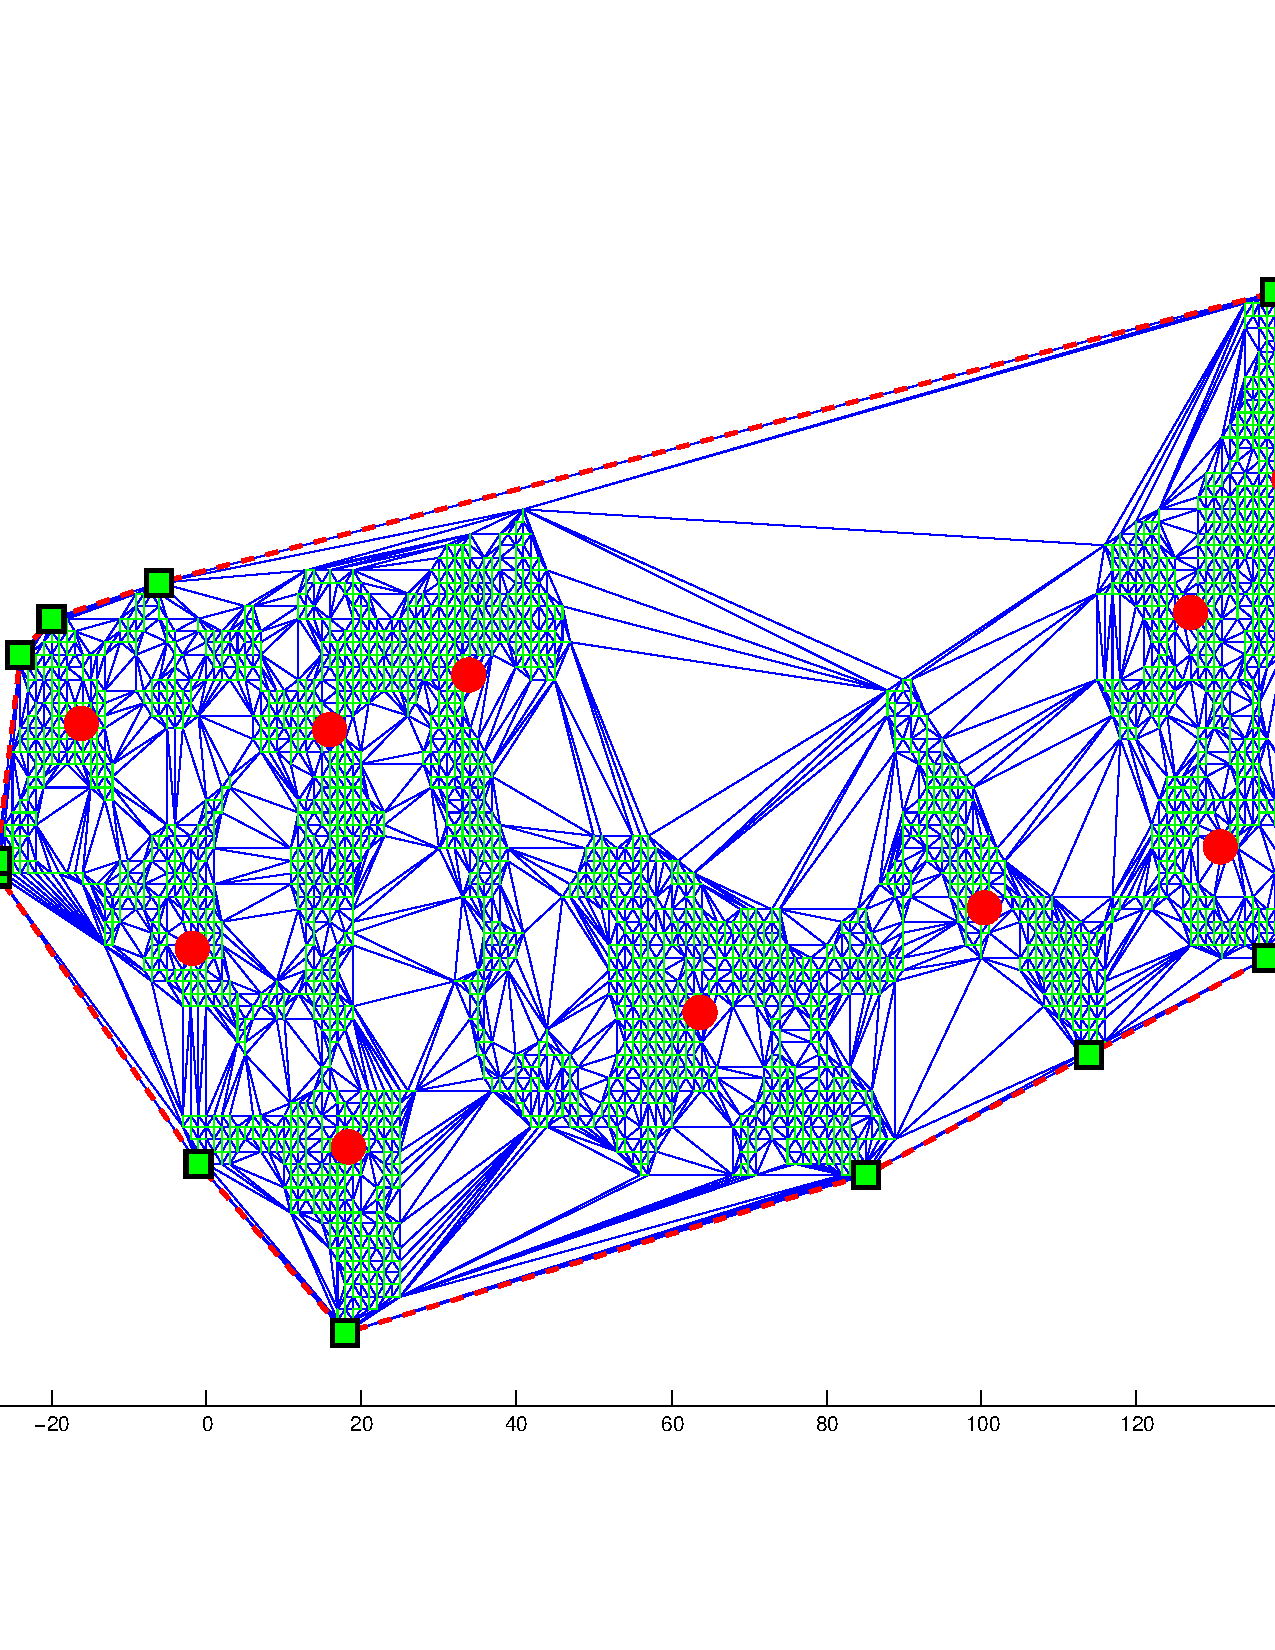
\includegraphics[width=8.0cm,height=8.0cm]{Figures/ClusteringRW/rw_10000_delauney_kmens_convex_hull.pdf}


\section*{The Matrix Exponential}
The matrix exponential of a matrix $\mat{A}$ is defined as
\begin{align*}
  e^{\mat{A}}
  &= \mat{I} + \mat{A} + \frac{\mat{A}^2}{2!} + \dots \\
  &= \sum_{k = 0}^\infty \frac{\mat{A}^k}{k!}.
\end{align*}

The Pade approximation to
$e^{\mat{A}}$ is
\begin{displaymath}
  e^{\mat{A}} \approx R(\mat{A}),
\end{displaymath}
with
\begin{align*}
  R_{pq} (\mat{A})
  &= (D_{pq}(\mat{A}))^{-1} N_{pq}(\mat{A}) \\
  \intertext{where}
  D_{pq}(\mat{A})
  &= \sum_{j=1}^p \frac{(p+q-j)! p!}{ (p+q)!j!(p-j)!}\, \mat{A}^j \\
  \intertext{and}
  N_{pq}(\mat{A})
  &= \sum_{j=1}^q \frac{(p+q-j)! q!}{ (p+q)!j!(q-j)!}\, \mat{A}^j.
\end{align*}
See \cite{Moler78nineteendubious} for a detailed accounting of this and other matters regarding the calculation of the matrix exponential.
%\citet{Moler78nineteendubious} \citep*{Moler78nineteendubious} \citep{Moler78nineteendubious} \citet*{Moler78nineteendubious}



\chapter{Appendix Numerical Software}
Computers are getting more powerful over time but size of the problems we're solving scales with the increased performance. Tools for acquiring and storing data are improving at an even faster pace than processors.  It turns out the communication is the real bottleneck to scaling many algorithms. The capacity of fast memory close to the computing resource (cache) grows very slowly in time.  Commodity hardware is now being used to deploy large distributed computing systems running Apache Hadoop and Spark. The possibility for computing on ever larger data sets is tantalizing for the machine learning community.
These notes discuss the a number of numerical computing libraries the author has used in various machine learning and image processing projects.  There is a lot of effort underway to integrate and distribute some of the algorithms in these libraries to the Hadooop ecosystem.

Many of the libraries discussed here are available in Matlab. Intel MLK \& IPP, Arpack, UMFPACK, and SDPA have been integrated in the autor's klMatrix library see the section on the KL Libraries below for specifics.

\section*{BLAS MLK \& Atlas}

\section*{Graphviz - Graph Visualization Software}
Graphviz ( http://www.graphviz.org ) is open source graph visualization software. Graph visualization is a way of representing structural information as diagrams of abstract graphs and networks. It has important applications in networking, bioinformatics,  software engineering, database and web design, machine learning, and in visual interfaces for other technical domains.

Graphviz is used to generate collaboration, inheritance, and call diagrams the KL documentation. There is an API that is used in the KL framework to facilitate graph visualization.

\section*{ARPACK}
ARPACK++ is an object-oriented version of the Fortran ARPACK package. ARPACK is designed to compute a few eigenvalues and eigenvectors of large scale sparse matrices and pencils via the Arnoldi process for finding eigenvalues called. These methods utilize Krylov Subspace Projections for iterative solution that avoids matrix multiplication.  ARPACK implements the implicit restarted Arnoldi method which reduces the storage requirements of the traditional Lanczos iteration for Hermitian matrices and Arnoldi iteration for general matrices.  The key to the Krylov method is to calculate the linear subspace of $\Real^{(n,n)}$ induced by span of the first m powers of the image of $b$ under a linear operator $A$, $\kappa_m(A,b) | A \in \mathbb R^{(n,n)}
b\ in \mathbb R^n = \{b, Ab (A)^2b, \ldots (A)^mb \}$.  This avoids direct matrix matrix operations when finding the first few eigenvector, eigenvalue pairs in a large system of linear
equations.

\section*{ATLAS}
Automatically Tuned Linear Algebra software.

\section*{METIS}
METIS is a software library for finite element analysis and graph partitions.  It also can be used to reduce the fill order of
sparse matrices.

\section*{SDPA}
SDPA is a software library for solving SDPs using on the Mehrotra-type predictor-corrector infeasible primal-dual interior-point method. It is implemented C++ language and utilizes the machine dependent BLAS such as Intel MKL, ATLAS. LAPACK routines are used for matrix computations.  Efficient methods to compute the search directions exploiting the sparsity of the data matrices are implemented. Sparse or dense Cholesky factorization for the Schur complemetn matrix is automatically selected. The calculation of the Schur complement
matrix is implemented in reentrant code. A sparse version of SDPA is available that uses METIS and SPOOLES libraries for finding a proper sparse structure of the problem.

\section*{SPOOLS}
SPOOLES is a library for solving sparse real and complex linear systems of equations. SPOOLES can factor and solve square linear systems of equations with symmetric structure, and it can compute multiple minimum degree, generalized nested dissection and multisection orderings of matrices with symmetric structure.  SPOOLES utilizes a variety of Krylov iterative methods. The preconditioner is a drop tolerance factorization.

\section*{SuperLU}
SuperLU ( http://crd-legacy.lbl.gov/~xiaoye/SuperLU/) is a general purpose library for the direct solution of large, sparse, nonsymmetric systems of linear equations on high performance machines. The library is written in C and is callable from either C or Fortran. The library routines will perform an LU decomposition with partial pivoting and triangular system solves through forward and back substitution. The LU factorization routines can handle non-square matrices but the triangular solves are performed only for square matrices. The matrix columns may be preordered (before factorization) either through library or user supplied routines. This pre-ordering for sparsity is completely separate from the factorization. Working precision iterative refinement subroutines are provided for improved backward stability. Routines are also provided to equilibrate the system, estimate the condition number, calculate the relative backward error, and estimate error bounds for the refined solutions.

\section*{SuiteSparse}
Tim Davis' ( http://www.cise.ufl.edu/~davis/welcome.html) collection of sparse matrix software.  Tim is also the curator of The University of Florida Sparse Matrix Collection (http://www.cise.ufl.edu/research/sparse/matrices/) a must see for anyone interested in sparse
matrices and visualization.

AMD: symmetric approximate minimum degree
BTF: permutation to block triangular form
CAMD: symmetric approximate minimum degree
CCOLAMD: constrained column approximate minimum degree
COLAMD: column approximate minimum degree
CHOLMOD: sparse supernodal Cholesky factorization and update/downdate
CSparse: a concise sparse matrix package
CXSparse: an extended version of CSparse
KLU: sparse$ LU$ factorization, for circuit simulation
LDL: a simple $LDL^T$ factorization
UMFPACK: sparse multifrontal $LU$ factorization
RBio: MATLAB toolbox for reading/writing sparse matrices
UFconfig: common configuration for all but CSparse
SuiteSparseQR: multifrontal sparse $QR$

\section*{SuiteSparse AMD}
AMD is a set of routines for pre-ordering a sparse matrix prior to numerical factorization. It uses an approximate minimum degree ordering algorithm to find a permutation matrix P so that the Cholesky factorization $PAP^\dag =LL^\dag$ has fewer (often much fewer) nonzero entries than the Cholesky factorization of A. The algorithm is typically much faster than other ordering methods and minimum degree ordering algorithms that compute an exact degree . Some methods, such as approximate deficiency [Rothberg and Eisenstat 1998] and graph-partitioning based methods [Hendrickson and Rothberg 1999; Karypis and Kumar 1998; Pellegrini et al. 2000; Schulze 2001] can produce better orderings, depending on the matrix. The algorithm starts with an undirected graph representation of a symmetric sparse matrix . Node $i$ in the graph corresponds to row and column i of the matrix, and there is an edge $(i,j)$ in the graph if $a_{ij}$ is nonzero. The degree of a node is initialized to the number of off diagonal non-zeros in row $i$, which is the size of the set of nodes adjacent to $i$ in the graph.

\section*{SuiteSparse UMFPACK}
UMFPACK is a set of routines for solving systems of linear equations, $Ax = b$, when $A$ is sparse and unsymmetric. It is based on the Unsymmetric-pattern MultiFrontal method. UMFPACK factorizes $PAQ$, $PRAQ$ and $PR^{-1}AQ$, into the product $LU$, where $L$ and $U$ are lower and upper triangular, respectively, $P$ and $Q$ are permutation matrices, and $R$ is a diagonal matrix of row scaling factors (or $R = I$ if row-scaling is not used). Both $P$ and $Q$ are chosen to reduce fill-in (new nonzeros in $L$ and $U$ that are not present in $A$). The permutation $P$ has the dual role of reducing fill-in and maintaining numerical accuracy (via relaxed partial pivoting and row interchanges). The sparse matrix $A$ can be square or rectangular, singular or non-singular, and real or complex (or any combination). Only square matrices $A$ can be used to solve $Ax = b$ or related systems. Rectangular matrices can only be factorized.

\section*{fftw}
fftw is a highly optimized library for calculating the discrete Fourier transform. \cite{G_ieeetrans_FFTW}.  Generally fftw performs better than Intel IPP.  fftw can be sped up by compiling with the Intel Compiler.

\section*{Simulation and modeling with the kl Software
Framework}Class, interaction and collaboration diagrams are presented below for a modeling framework implemented by the author. The framework is implemented in C++.  The simulation of various univariate and multivariate random number generators along with the distribution tests from the CDHC library are included as well.
Features of this framework include:
\begin{itemize}
\item utilizing optimized BLAS libraries
\item the up to date methods for univariate random number generation
\item wrappers for Intel performance primitives and GSL
\item multiple memory management facilities
\end{itemize}
We will use the term $EPDF_X$ to mean the empirical probability density function. There are a variety of univariate tests to help determine which parametric distribution your data belongs to. These fall under the category of Goodness of Fit testing. For a parametric family the null hypothesis $H_o : X=_d p(x| \theta)$ is tested against the alternative that $X$ does not belong to the family $p(x|\theta)$ There are also family of test to determine whether two $EPDF$'s come from the same distribution. 

\section*{Bushido of Software Engineering}

The end result does not matter....
The users don't matter....
The success of the product does not matter....
The code alone and nothing but the code matters....
To thine own code alone shalt thou be true.

If the code does only and exactly what you intended it to, that is Zen.
If the code is also as fast as you want it to be, that is Zen.
If the code is also as clean as you want it to be, that is Zen.
If the code is also as readable as you want it to be, that is Zen.

But you must intend strongly, you must measure critically, indent perfectly and comment willingly, other wise it is not Zen.


\section*{Zen of Modelling}

- Your model should have some theoretical basis.
- Your model, when simulated, should produce outcomes with a similar density to the observed values. Similarly, your model should not place weight on the impossible (like negative quantities, or binary outcomes that aren’t binary). It should place non-zero weight on possible but unlikely outcomes.
- Think deeply about what is a random variable and what is not. A good rule of thumb: random variables are those things we do not know for certain out of sample. Your model is a joint density over the random variables.
- You never have enough observations to distinguish one possible data generating process from another process that has different implications. You should model both, giving both models weight in decision-making.
- The point of estimating a model on a big dataset is to estimate a rich model (one with many parameters). Using millions of observations to estimate a model with dozens of parameters is a waste of electricity.
- Unless you have run a very large, very well-designed experiment, your problem has unobserved confounding information. If this problem does not occupy a lot of your time, you are doing something wrong.
Fixed effects normally aren’t. Mean reversion applies to most things, including unobserved information. Don’t be afraid to shrink.
- Relationships observed in one group can almost always help us form better understanding of relationships in another group. Learn and use partial pooling techniques to benefit from this.
- For decision-making, your estimated standard deviations are too small; your estimated degrees of freedom are too big, or your have confused one for the other. Remember, the uncertainty produced by your model is the amount of uncertainty you should have if your model is correct and the process you are modeling does not change.
- You always have more information than exist in your data. Be a Bayesian, and use this outside information in your priors.


\section*{Model Workflow}

1. Plot your data

2. Write down what you know both in and out of sample, and what you only know in sample.
As I wrote in my rules of thumb, you need to have a very clear idea of what the random variables are in your model. Random variables are simply those variables whose values are in part due to chance. For most modeling purposes, our random variables are the things we don’t know for sure out of sample. These might include model parameters, latent variables, predictions, etc. [Edit: I don't mean literally that model parameters are random; it's our understanding of them which has uncertainty].
A common problem occurs when the modeler uses a random variable as a predictive feature in a model but does not explicitly model it. For instance they might build a model that looks a bit like
Salest=f(Weathert,Day of the weekt)+effort

Next, when called on to make a prediction, the modeler uses forecasts for weather to generate predictions for sales, but without taking into account the uncertainty around weather (a random variable). As for the day of the week, this is not a random variable and so we don’t have to model it. Any forecasts conditioned on random variables without taking into account their uncertainty will be far too precise.
The reason we should write down what the random variables are in the model is because this is precisely what we are going to model.
3. Build a generative model of those things that you don’t know out of sample.
In this step, we ask ourselves: what is a plausible process that could generate the outcomes that we observe? For instance, if we think that a normal linear regression model with coefficients β and covariates X and residual standard deviation σ is suitable, our generative model would be
yi∼N(Xβ,σ)
Or we might consider a normality assumption to be too strong, and use a “fat-tailed distribution” instead
yi∼Student's t(ν,Xβ,σ)
Or perhaps our outcome yi comes from two distribtuions, each with a different probability (as in this post). Or it could be binary, or count data, or strictly positive data, or multimodal data, etc., in which we would choose different distributions still.
Note that the examples above are extremely simple models—you should almost always start with simple models and build up in complexity. As your model grows in complexity, the value to performing the fake data exercise in steps 4 and 5 grows.
After defining the generative model, you should assign some priors to all the unknowns—in this case, the parameters ν, β, and σ. These priors should give weight to plausible values of the parameters of the model, and no weight to impossible values. For instance, ν is restricted to be >1 and σ has to be positive. Priors for those parameters should not put weight on values outside that range.
4. Draw some data from the generative model with some known parameters drawn from the prior.
We have a generative model for our data—a way to simulate plausible values for y given X—and priors for the parameters.
The next step is to draw some values from a prior, which we treat as being “known” values of the parameters. After doing this we have values for X, and “known” values for ν, β and θ, so we can simulate some fake data by drawing observations from the generative model in step 3.
Why should we simulate some fake data? First, it gives us an idea of whether our model puts weight on impossible outcomes—we don’t want to use a model that does that! But more importantly, this (often skipped) step makes us be very explicit about all the assumptions in the model, and guides us to the estimation in the next step.
5. Estimate the model on the fake data. Can you recover the parameters? Is the model identified?
Before taking your estimation model to real data, you should always try estimating the model on the fake data you simulated in step 4. Why do this? First, you know the values of the parameters for that data. So you should check to see that when you estimate your model on fake data you can recapture the known values. If your model is unable to recapture known parameters with fake data, it will definitely estimate the wrong parameter values using real data.
6. Estimate the model on real data
If your model is able to recapture known parameter values, it’s time to estimate the model on real data.
Often people jump to this step without performing 4 and 5 first, and get funny results. (I know this because some of these people are my friends and I receive a few emails a week about precisely this problem). Gelman’s folk theorem is “it’s probably not the computer. It’s probably your model.” and this is almost always the case here.
7. Check for model convergence
Sometimes, especially for big, loosely-identified models, you might not be getting very good samples from your posterior. One great tool in R for exploring pathologies in sampling is shinystan (available here), which provides a web interface to your MCMC fits.
If you have poor convergence or pathologies in sampling, this can often be fixed by reparameterizing your model. Reparameterizing a model is simply a way of expressing the same model in a way that your posterior has a more regular shape (and so is easier to sample from).
8. Posterior predictive checking and inference
Now we know that the model has been built well and is estimating fine. But was it the right model in the first place? Posterior predictive checking is a very useful method for answering this question. The aim is to check to see if, when simulated, the model generates predictions that have a similar distribution to the observed data, after taking into account uncertainty in the model parameters.
An example of this is below, from some recent work of mine modeling micro-loan repayments in Sub-Saharan Africa.




9 Iterate!
We have just built a fairly simple model, but now we have it working, and we probably have a good idea what’s wrong with it. At this point we can afford to go back to step 3 and build up a more complex model, knowing that if anything breaks (or a deadline approaches), we have a well-built, well-checked model ready to go. 





\setlinespacing{1.0}
%\bibliographystyle{amsplain}
\bibliographystyle{plainnat}
\bibliography{thebibliography}

\end{document}
